\documentclass[11pt,letterpaper]{article}
\usepackage{style}

%% ------- INICIA DOCUMENTO ------
\begin{document}
\begin{titlepage}
\begin{center}
\begin{LARGE}
INSTITUTO POLITÉCNICO NACIONAL\\
\vspace*{0.15in}
ESCUELA SUPERIOR DE CÓMPUTO\\
\end{LARGE}
\vspace*{1.0in}
\begin{Large}
%% NOMBRE DE LA PRÁCTICA O EXAMEN
\textbf{TÉCNICAS DE CRUZA 1} \\  
\end{Large}
\vspace*{0.2in}
\begin{large}
\textit{Práctica 6}\\
\end{large}
\vspace*{1.0in}
\begin{large}
%% INTEGRANTES	
Dominguez de la Rosa Bryan\\
\vspace*{2.0in}
GRUPO 3CM5\\
\vspace*{0.2in}
Profesor: Morales Güitron Sandra Luz\\
\vspace*{1.5in}
\today
\vspace*{0.3in}
\end{large}
\rule{150mm}{0.1mm}\\

\end{center}
\end{titlepage}

%% --------- COMIENZA EL DESARROLLO DEL DOCUMENTO --------

\section*{Introducción}
En general, se necesitan los cinco componentes basicos siguientes para
implementar un AG que resuelva un problema cualquiera:

\begin{enumerate}
	\item Una representacion de soluciones potenciales al problema.
	\item Una forma de crear una poblacion inicial de soluciones potenciales (esto
	se efectua normalmente de manera aleatoria, pero tambi en pueden usarse
	metodos determinísticos).
	\item Una funcion de evaluación que juega el papel del ambiente, calificando a
	las soluciones producidas en terminos de su “aptitud”.
	\item Operadores geneticos que alteran la composición de los descendientes (normalmente se usan la cruza y la mutacion).
	\item Valores para los diversos parametros utilizados por el algoritmo genético
	(tamaño de la población, probabilidad de cruza y mutación, número máximo
	de generaciones, etc.)
\end{enumerate}

La representación tradicional usada para codificar un conjunto de soluciones es el esquema binario en el cual un cromosoma es una cadena. 

\section*{Contenido}

Se realizaron 4 representaciones de individuos:
\begin{itemize}
	\item Binaria.
	\item Grey.
	\item Reales.
	\item Enteros.
\end{itemize}

En cada una, se generaron 10 individuos de manera aleatoria, para observar diferentes ejemplos.

Para compilar cada programa se ejecuta la siguiente línea, sustituyendo el parámetro \textit{name} con el nombre del programa:

\begin{center}
	\textbf{g++ \textit{name.cpp} -o \textit{name}}
\end{center}
	
Una vez compilado el código, pasamos a la ejecución, para lo cuál usamos el comando  \textbf{./\textit{name}}.\\

La representación de individuos generados aleatoriamente se muestran a continuación:\\

\subsection*{Representación binaria}

\begin{figure}[H]
	\centering
	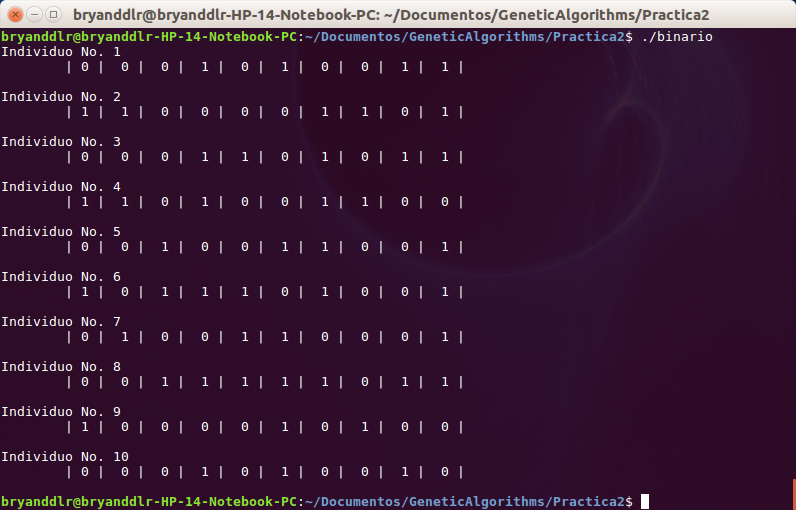
\includegraphics[scale = 0.5]{images/ej1}
\end{figure}

\subsection*{Representación binaria codificada en grey}
\begin{figure}[H]
	\centering
	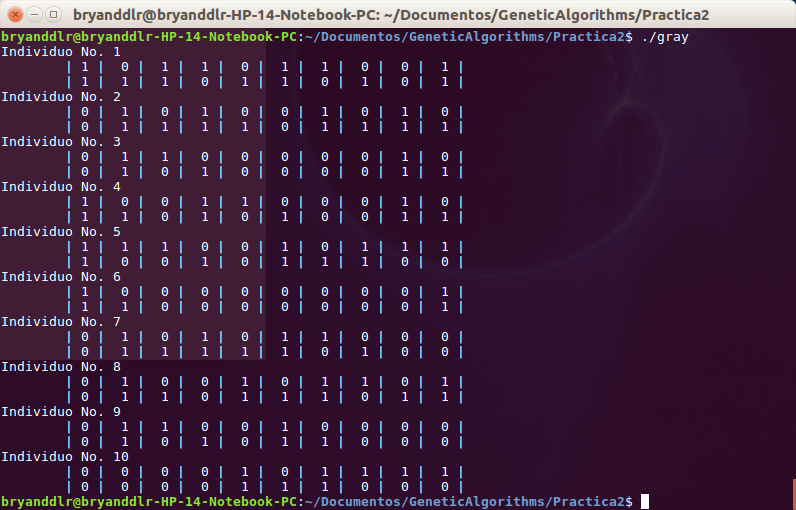
\includegraphics[scale = 0.5]{images/ej2}
\end{figure}

\subsection*{Representación real}
\begin{figure}[H]
	\centering
	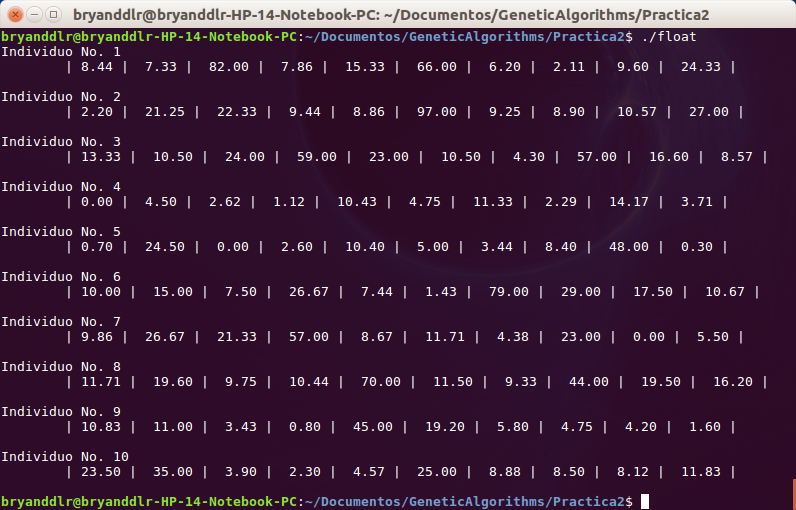
\includegraphics[scale = 0.5]{images/ej3}
\end{figure}

\subsection*{Representación entera}
\begin{figure}[H]
	\centering
	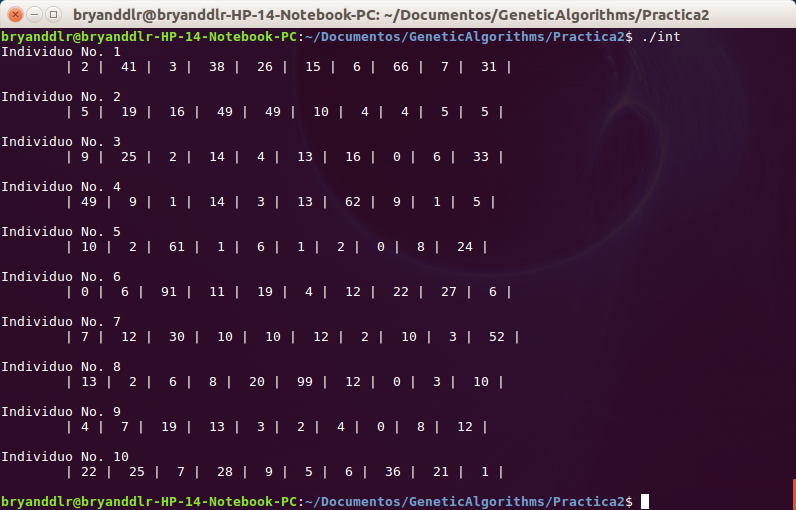
\includegraphics[scale = 0.5]{images/ej4}
\end{figure}

\section*{Conclusión}


\end{document}


